\documentclass[a4paper,titlepage,twoside,12pt,leqno]{article}

\usepackage[]{fontspec}
\usepackage{xltxtra}
\usepackage[monogreek]{xgreek}

\newcommand{\en}[1]{\setlanguage{american}#1\setlanguage{monogreek}} % Για υφενώσεις στα αγγλικά

\defaultfontfeatures{Mapping=tex-text%, Scale=MatchLowercase}
} 

% Γραμματοσειρά
\setmainfont[Mapping=tex-text]{DejaVu Sans}


\usepackage{longtable} % για έναν μεγάλο πίνακα
\usepackage{graphicx, array, blindtext}

\title{Αναλυτικό εγχειρίδιο αναφοράς για το ηλεκτρονικό θεματικό πάρκο σε μεσαιωνική καστροπολιτεία}
\author{Αναγνωστόπουλος Βασίλης-Θάνος, Κατσής Γιώργος}
\date{}

\begin{document}

\maketitle
\tableofcontents
\listoffigures
\listoftables
\newpage

\section{Εισαγωγή}

%Στα εγχειρίδια αυτά παρουσιάζεται η σύνταξη όλων των εντολών του προγράμματος. Σε αυτά τα εγχειρίδια ανατρέχει ένας χρήστης για να βρει την σύνταξη της οποιασδήποτε εντολής. Ο στόχος των εγχειριδίων αυτών είναι να καλύψουν πλήρως τη λειτουργία ενός προγράμματος και όχι να εκπαιδεύσουν το χρήστη. Αυτά τα εγχειρίδια χρησιμεύουν σε όλους τους χρήστες, είτε αυτοί είναι καινούριοι είτε παλαιότεροι οπότε γνωρίζουν λίγο πολύ τη λειτουργία του προγράμματος.

Το συγκεκριμένο πρόγραμμα προορίζεται για την αλληλεπίδραση των ενοίκων του μεσαιωνικού κάστροδιαμερίσματος με τις διάφορες συσκευές και υπηρεσίες που διαθέτει το διαμέρισμα του και η καστοπολιτεία. Συγκεκριμένα μέσα αυτού του προγράμματος μπορείτε να διαχειριστεί τις παρακάτω συσκευές:

\begin{itemize}
\item την πόρτα του διαμερίσματος του (βλέπε σελ. \ref{pisina})
\item Πισίνα (βλέπε σελ. \ref{pisina})
\item Να βάλουμε και άλλες συσκευές.

\end{itemize}

\section{Πλοήγηση στην εφαρμογή}

\emph{τα εγχειρίδια αυτά σε τί γλώσσα να είναι γραμμένα. Εννοώ στον ενικό, στον πληθυντικό σε α, β ,γ πρόσωπο... Τί στυλ να έχει;;; Ακόμα τί κεφάλαια να περιλαμβάνονται.}

Η πρώτη οθόνη της εφαρμογής είναι για την επιλογή του κατάλληλου μενού για την αλληλεπίδραση με την καστροπολιτεία. Στα δεξιά του παραθύρου φαίνονται σημαίες από χώρες που πατώντας και πατώντας κάποια σημαία αλλάζει η γλώσσα των μηνυμάτων που εμφανίζονται στην εφαρμογή.

\emph{Να μπει πίνακας για να τα επεξηγεί όλα και όχι ένα ένα για να μειωθεί ο χώρος που χρειάζονται}

Στα αριστερά της εφαρμογής φαίνονται τα εικονίδια επιλογών καθώς και ένα μικρό κείμενο το οποίο επεξηγεί τί κάνει το καθένα (βλ. σχήμα \ref{fig:menu:general})

\begin{figure}
\begin{center}
\resizebox*{10.5cm}{!}{
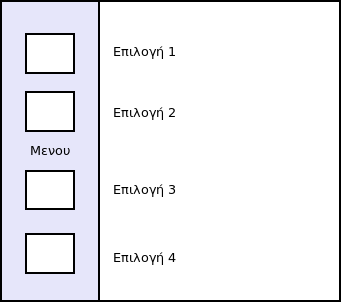
\includegraphics{images/menu.png}}
\caption{Το γενικό μενού (σε αφηρημένη μορφή).}
\label{fig:menu:general}
\end{center}
\end{figure}

Αναλυτικά το εικονίδιο με του δύο παλαιστές σούμο (λέμε τώρα...) κάνει αυτό και αυτό (βλέπε σχήμα \ref{fig:icon:})

\begin{figure}
\begin{center}
\resizebox*{10.5cm}{!}{
\rule{0.4\textwidth}{0.3\textwidth}}
\caption{Το εικονίδιου για την μετάβαση σε .....}
\label{fig:icon:}
\end{center}
\end{figure}

Το άλλο με το πεντάφυλο κάνει τάδε ...

\emph{Εδώ να βάλουμε φωτό από τα εικονίδια και τι κάνει το καθένα}

Όταν πατηθεί κάποιο εικονίδιο τότε μεταβαίνουμε σε ένα νέο παράθυρο το οποίο αλλάζει ανάλογα με την επιλογή, όμως το μενού με τα εικονίδια στα αριστερά θα παραμένει έτσι ώστε να είναι δυνατή η εναλλαγή μεταξύ των μενού γρήγορα να είμαστε υποχρεωμένοι να γυρίσουμε στην αρχική οθόνη.

\section{Παραγγελία αντικειμένων}
\label{paraggelia}

Σε αυτό το μενού μπορούμε να παραγγείλουμε προϊόντα από την καφετέρια-εστιατόριο της καστροπολιτείας μας. Για να εισέλθουμε σε αυτό το μενού θα πρέπει να πατήσουμε το εικονίδιο με τους (περιγραφή) από το κεντρικό μενού (βλ. σχήμα \ref{}).

\begin{figure}
\begin{center}
\resizebox*{10.5cm}{!}{
\rule{0.4\textwidth}{0.3\textwidth}}
\caption{Το εικονίδιου για την μετάβαση σε .....}
\label{fig:icon:}
\end{center}
\end{figure}

Αρχικά εμφανίζονται οι κατηγορίες των αντικειμένων των οποίων μπορούμε να αγοράσουμε από την καφετέρια-εστιατόριο της καστροπολιτείας μας (βλ. σχήμα \ref{})

\begin{figure}
\begin{center}
\resizebox*{10.5cm}{!}{
\rule{0.4\textwidth}{0.3\textwidth}}
\caption{Το εικονίδιου για την μετάβαση σε .....}
\label{fig:icon:}
\end{center}
\end{figure}

Επιλέγοντας μία κατηγορία "ανοίγουν" και εμφανίζονται τα προϊόντα σε αυτή την κατηγορία. Επιλέγοντας ένα από τα αντικείμενα ανοίγει μία νέα φόρμα που περιγράφει αναλυτικά το αντικείμενο (βλ. σχήμα \ref{}).

\begin{figure}
\begin{center}
\resizebox*{10.5cm}{!}{
\rule{0.4\textwidth}{0.3\textwidth}}
\caption{Το εικονίδιου για την μετάβαση σε .....}
\label{fig:icon:}
\end{center}
\end{figure}

\section{Διαχείριση τάφρου-πισίνας}
\label{pisina}

Σε αυτό το μενού μπορούμε να διαχειριστούμε την πισίνα-τάφρο του διαμερίσματος

\section{Διαχείριση ηλεκτρονικών συσκευών}
\label{syskeuves}


\end{document}
